\documentclass[11pt,a4paper]{article} 
\usepackage{amssymb}
\usepackage[shortlabels]{enumitem}
\usepackage[fleqn]{amsmath} 
\usepackage{relsize}
\usepackage{graphicx}
\usepackage[super]{nth}
\usepackage{hyperref, url}
\usepackage[margin=2cm, top=2cm]{geometry}
\graphicspath{{./img/}}
\newcommand\setItemNumber[1]{\setcounter{enumi}{\numexpr#1-1\relax}}
\newcommand*{\mybox}[1]{\framebox{#1}}
\newcommand{\tuple}[1]{$\langle #1 \rangle$} 
\newcommand{\stuple}[1]{$\langle$#1$\rangle$} % ordered pair with strings inside
\newcommand{\forceindent}{\leavevmode{\parindent=1em\indent}}

\title{\bf Homework 1\\[1ex]
\rm\normalsize CS250 Discrete Structures I, Winter 2020 }
\date{\normalsize Due: April 26, 2020}
\author{\normalsize Armant Touche}

\begin{document} 
\vspace{0cm}\maketitle 
	\paragraph{Homework Exercises} Chapter 2: Sequences
	
	\subparagraph{Problem 1} 2.1 Describing Sequences (pg. 135-147)\\
			
		From section 2.1 in the textbook, complete exercises 2, 3, 7, 10, 13, 18

        \begin{enumerate}

            %2
            \setItemNumber{2}
            \item For each sequence given below, find a closed formula for $a_n$, the $n$th term of the sequence (assume the first terms are $a_0$ ) by relating it to another sequence for which you already know the formula. In each case, briefly say how you got your answers.
                \begin{enumerate}
                    \item 4, 5, 7, 11, 19, 35, . . .\\
                        I noticed that the difference between each number had a factor of power to two where the the first two number's difference was 1, plus 3 implied, then next pair was 2, 4, 8, and so on. So $a_n = 3 + 2^n;\;\;(a_n)_{n\geq 0}$ is my closed formula.
                    \item 0, 3, 8, 15, 24, 35,. . .\\
                        Like (a), I notice a trend in the differences between each number and this sequence reminded me of the partial sum sequence because the recurring difference between each pair of numbers was two. So I think $a_n = n(n + 2);\;(a_n)_{n\geq 0}$ is the answer.
                    \item 6, 12, 20, 30, 42, . . .\\
                        This sequence resemble the square sequence so $a_n = a_{n + 1} + {n + 1}$ where $n\in\mathbb{N}\land a_{n\geq 1}$
                    \item 0, 2, 7, 15, 26, 40, 57, . . . (Cryptic Hint: these might be called “house numbers”)
                        
                \end{enumerate}

            %3
            \item Write out the first 5 terms (starting with $a_0$ ) of each of the sequences described below. Then give either a closed formula or a recursive definition for the sequence (whichever is NOT given in the problem).
                \begin{enumerate}
                    \item $a_n = \frac{1}{2}(n^2 + n)$  \\
                        $a_0 = 0\\a_1 = 1\\a_2 = 3\\a_3 = 6\\a_4 = 10$\\
                        $a_{n+1} = a_n +n$ with $a_0 = 0$
                    \item $a_n = 2a_{n - 1} - a_{n - 2}$ with $a_0 = 0$ and $a_1 = 1$\\
                        $a_2 = 2\\a_3 = 3\\a_4 = 4\\a_5 = 5\\a_n = n$ is the closed formula
                    \item $a_n = na_{n - 1}$ with $a_0 = 1$\\
                        $a_0 = 1\\a_1 = 1\\a_2 = 2\\a_3 = 6\\a_4 = 24\\a_5 = 120$\\
                        The closed formula is $a_n = n!$ is the closed formula 56                 
                \end{enumerate}

            %7
            \setItemNumber{7}
            \item Write out the first few terms of the sequence given by $a_1 = 3$; $a_n = 2a_{n - 1} + 4$. Then find a recursive definition for the sequence 10, 24, 52, 108, . . .\\
                $a_1 = 3\\ a_2 = 10\\ a_3 = 24\\ a_4 = 52\\ a_5 = 108$\\ The rec. def. for the sequence just listed is $a_n = 2a_{n - 1} + 4$ with $a_1 = 10$


            %10
            \setItemNumber{10}
        \item Show that $a_n = 2^n - 5^n$ is also a solution to the recurrence relation $a_n = {7a_{n - 1}} - {10a_{n - 2}}$. What would the initial conditions need to be for this to be the closed formula for the sequence?\\
            $a_0 = 2^0 - 5^0 = 0\\a_1 = 2^1 - 5^1 = -3\\a_2 = 2^2 - 5^2 = -21\\a_3 = 2^3 - 5^3 = -117$\\
            So to prove the recurrence, the initial condition needs to be $a_3 = -117$ for the closed formula and recurrence relation to exist.


            %13
            \setItemNumber{13}
        \item Use summation ($\Sigma$) or product ($\Pi$) notation to rewrite the following
            \begin{enumerate}

                \item $2 + 4 + 6 + 8 + ... + 2n\\\\ = {\mathlarger{\sum}}_{k=1}^{n}\;2k$\\
                \item $1 + 5 + 9 + 13 + ... + 425\\\\ = 4{\mathlarger{\sum}}_{k=1}^{107}(k-1)+1$\\
                \item $1 + \frac{1}{2} + \frac{1}{3} + \frac{1}{4} + ... + \frac{1}{50}\\\\= {\mathlarger{\sum}}_{k=1}^{50}\frac{1}{i}$\\
                    \item $2\cdot 4\cdot 6\cdot ... \cdot2n\\\\= 2{\mathlarger{\prod}}_{k=1}^n k$\\
                    \item $(\frac{1}{2})(\frac{2}{3})(\frac{3}{4})...(\frac{100}{101})\\\\={\mathlarger{\prod}}_{k=1}^{100}\frac{k}{k+1}$
            \end{enumerate}

            %18
            \setItemNumber{18}
            \item When bees play chess, they use a hexagonal board like the one shown below. The queen bee can move one space at a time either directly to the right or angled up-right or down-right (but can never move leftwards). How many different paths can the queen take from the top left hexagon to the bottom right hexagon? Explain your answer, and this relates to the previous question. (As an example, there are three paths to get to the second hexagon on the bottom row.)

            \begin{center}
            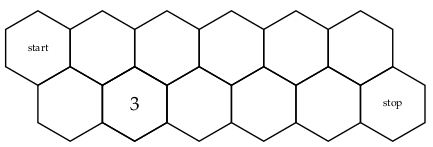
\includegraphics[width=.5\textwidth]{hw6_graphic1}
            \end{center}

            I noticed the pattern had a close formula $a_n = a_{n-1} + b_n$ and with a total number of path being 144 paths. This is a pascal's triangle problem if I were to cut the board in half and calculate using recurrence relation, $b_1 = 3\;\;\text{and}\; a_0 = 1$. This problem is tricky but I think n = 6  which gives us 144 paths using this approach.
	
        \end{enumerate}

	\subparagraph{Problem 2} 2.2 Arithmetic and Geometric Sequences (pg. 148-159)\\
	
		From section 2.2 in the textbook, complete exercises 1, 3, 4, 13, 15
	
        \begin{enumerate}

            %1
            \item Consider the sequence 5, 9, 13, 17, 21, . . . with $a_1 = 5$
                \begin{enumerate}

                \item Give a recursive definition for the sequence.\\
                $a_ = a_{n-1} + 4$ when $a_1 = 5$
                \item Give a closed formula for the nth term of the sequence.\\
                $a_n = 5 + 4(n-1)$
                \item Is 2013 a term in the sequence? Explain.\\
                $$2013 = 5 + 4(n - 1)$$
                $$2013 = 5 + 4n - 4$$
                $$2012 = 4n$$
                $$\frac{2012}{4} = n$$
                $$n = 503$$
                Yes, using some algebra, we can validate that 2013 is the \nth{503} term.\\
                \item How many terms does the sequence 5, 9, 13, 17, 21, . . . , 533 have\\
                    $$533 = 5 + 4(n - 1)$$
                    $$533 = 5 + 4n - 1$$
                    $$\frac{533}{4} = n$$
                    $$n = 133$$
                    533 is the \nth{133} term so 133 terms in total
                \item Find the sum: 5 + 9 + 13 + 17 + 21 + · · · + 533. Show your work.\\
                    $$4\cdot{\mathlarger{\sum}}_{k=1}^{133}(k - 1) + 5 = 3577$$
                \item Use what you found above to find $b_n$ , the $n$th term of 1, 6, 15, 28, 45, . . ., where $b_0 = 1$
                    $$b_n = \frac{(4n^2 + 6n)}{2} + 1$$
                \end{enumerate}


            %3
            \setItemNumber{3}
            \item Consider the sum 4 + 11 + 18 + 25 + · · · + 249.
                \begin{enumerate}
                    \item How many terms (summands) are in the sum?\\
                        Closed formula:\\
                        $$a_n = 7n + 4$$
                        Next, we solve this question by setting the formula equal to 249 and solve for number of terms.\\
                        $$249 = 7n + 4$$
                        $$n = 36$$
                        There are 36 terms in the sum.\\
                    \item Compute the sum using a technique discussed in this section.\\
                        $${\mathlarger{\sum}}_{k=0}^{35}7k + 4 = \frac{(36)(253)}{2}$$
                        $$ n = 4554$$
                \end{enumerate}

            %4
            \item Consider the sequence 1, 7, 13, 19, . . . , $6n + 7$.
                \begin{enumerate}
                    \item How many terms are there in the sequence? Your answer will be in terms of $n$.\\
                        $n + 2$ terms. ${\mathlarger{\sum}}_{k = -1}^{n} 6n +7$.
                    \item What is the second-to-last term?\\
                        Since $6n + 1$ is six less than the last terms so $(7 -1) = 6$.
                    \item Find the sum of all the terms in the sequence, in terms of n.\\
                        $$ 6\cdot{\mathlarger{\sum}}_{k=-1}^{n}n + {\mathlarger{\sum}}_{k=-1}^{n}7 = \frac{(6n+8)(n+2)}{2}$$

                \end{enumerate}


            %13
            \setItemNumber{13}
            \item If you have enough toothpicks, you can make a large triangular grid. Below, are the triangular grids of size 1 and of size 2. The size 1 grid requires 3 toothpicks, the size 2 grid requires 9 toothpicks.

            \begin{center}
            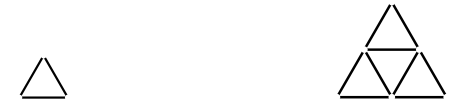
\includegraphics[width=.5\textwidth]{hw6_graphic2}
            \end{center}

                \begin{enumerate}
                    \item Let $t_n$ be the number of toothpicks required to make a size n triangular grid. Write out the first 5 terms of the sequence $t_1, t_2, ...$.
                        $t_1 = 3\\t_2 = 9\\t_3 = 9\\t_4 = 30\\t_5 = 45$
                    \item Find a recursive definition for the sequence. Explain why you are correct
                        $$t_n = t_{n-1} + \frac{6n}{2};\;\;n\geq 2$$
                        Since $t_0 = 1$ highlights that this sequence is triangular number sequence but our base case is $t_1 = 3$.
                    \item Is the sequence arithmetic or geometric? If not, is it the sequence of partial sums of an arithmetic or geometric sequence? Explain why your answer is correct.
                        $t_n$ is a partial sums sequence since the $n$th term in an given indice is the sum of the first $n$ term (i.e. $t_{n-1} + t$, where $t_n$ refers to the number of toothpicks at any given height which equals total number of toothpicks.
                    \item Use your results from part (c) to find a closed formula for the sequence. Show your work.
                        $$(t_n)_{n\geq 1} = \frac{6n + 3(n - 1)n}{2}$$
                        3 toothpicks are needed intially
                \end{enumerate}

            %15
            \setItemNumber{15}
            \item Here is a surprising use of sequences to answer a counting question: How many license plates consist of 6 symbols, using only the three numerals 1, 2, and 3 and the four letters a, b, c, and d, so that no numeral appears after any letter? For example, “31ddac” and “12321” are acceptable license plates, but “13ba2c” is not.
                \begin{enumerate}
                    \item First answer this question by considering different cases: how many of the license plates contain no numerals? How many contain one numeral, etc.
                        $$A = \{a, b, c, d\}$$
                        $$B = \{1, 2, 3 \}$$
                        License plates w/ no numerals = $|A|^6\cdot |B|^0 = 4096$\\
                        License plates w/ one numerals = $|A|^5\cdot |B|^1 = 3072$\\
                        License plates w/ $n$ numerals = $|A|^{(6 - n)} \cdot |B|^{n} =$ number of possible license plates outcomes.\\
                        Closed formula:\\
                        $$ a_n = 4^{6-n}\cdot 3^{n};\;\;n\geq 0$$ 
                    \item Now use the techniques of this section to show why the answer is $4^7 - 3^7$.\\\\

                        \textit{Proof}. First let's hightlight:\\\\
                        $n_0 = 0 \rightarrow 4096$ license plates\\
                        $n_1 = 1 \rightarrow 3072$ license plates\\
                        $n_2 = 2 \rightarrow 2304$ license plates\\
                        $n_3 = 3 \rightarrow 1728$ license plates\\
                        $n_4 = 4 \rightarrow 1296$ license plates\\
                        $n_5 = 5 \rightarrow 972$ license plates\\
                        $n_6 = 6 \rightarrow 729$ license plates\\\\
                        So total sum of possibilities is :\\
                        $${\mathlarger{\sum}}_{k=0}^{6}4^{6-n}\cdot 3^n = 14197 = 4^7 - 3^7$$
                        Since this is a geometric sequence, there is a ratio of the seven in the exponents balances out the ratio. 

                \end{enumerate}

        \end{enumerate}
	
	
		
\end{document}
